%%%%%%%%%%%%%%%%%%%%%%%%%%%%%%%%%%%%%%%%%%%%%%%%%%%%%%%%%%%%%%%%%%%%%%
% LaTeX Example: Project Report
%
% Source: http://www.howtotex.com
%
% Feel free to distribute this example, but please keep the referral
% to howtotex.com
% Date: March 2011 
% 
%%%%%%%%%%%%%%%%%%%%%%%%%%%%%%%%%%%%%%%%%%%%%%%%%%%%%%%%%%%%%%%%%%%%%%
% How to use writeLaTeX: 
%
% You edit the source code here on the left, and the preview on the
% right shows you the result within a few seconds.
%
% Bookmark this page and share the URL with your co-authors. They can
% edit at the same time!
%
% You can upload figures, bibliographies, custom classes and
% styles using the files menu.
%
% If you're new to LaTeX, the wikibook is a great place to start:
% http://en.wikibooks.org/wiki/LaTeX
%
%%%%%%%%%%%%%%%%%%%%%%%%%%%%%%%%%%%%%%%%%%%%%%%%%%%%%%%%%%%%%%%%%%%%%%
% Edit the title below to update the display in My Documents
%\title{Project Report}
%
%%% Preamble
\documentclass[paper=a4, fontsize=11pt]{scrartcl}
\usepackage[T1]{fontenc}
\usepackage{fourier}
\usepackage{hyperref}

\usepackage[english]{babel}															% English language/hyphenation
\usepackage[protrusion=true,expansion=true]{microtype}	
\usepackage{amsmath,amsfonts,amsthm} % Math packages
\usepackage[pdftex]{graphicx}	
\usepackage{url}
\newcommand{\git}{\href{https://github.com/arnthorg/HVR2-2016/}{\underline{GitHub} }}

%%% Custom sectioning
\usepackage{sectsty}
\allsectionsfont{\centering \normalfont\scshape}


%%% Custom headers/footers (fancyhdr package)
\usepackage{fancyhdr}
\pagestyle{fancyplain}
\fancyhead{}											% No page header
\fancyfoot[L]{}											% Empty 
\fancyfoot[C]{}											% Empty
\fancyfoot[R]{\thepage}									% Pagenumbering
\renewcommand{\headrulewidth}{0pt}			% Remove header underlines
\renewcommand{\footrulewidth}{0pt}				% Remove footer underlines
\setlength{\headheight}{13.6pt}


%%% Equation and float numbering
\numberwithin{equation}{section}		% Equationnumbering: section.eq#
\numberwithin{figure}{section}			% Figurenumbering: section.fig#
\numberwithin{table}{section}				% Tablenumbering: section.tab#


%%% Maketitle metadata
\newcommand{\horrule}[1]{\rule{\linewidth}{#1}} 	% Horizontal rule

\title{
		%\vspace{-1in} 	
		\usefont{OT1}{bch}{b}{n}
		\normalfont \normalsize \textsc{Háskólinn í Reykjavík} \\ [25pt]
		\horrule{0.5pt} \\[0.4cm]
		\huge Einkenning skynjara og mælaborð\\ í Formúlubíl HR \\
		\horrule{2pt} \\[0.5cm]
}
\author{
		\normalfont 								\normalsize
        Arnþór Gíslason\\[-3pt]		\normalsize
        Sigurður Gunnar Sigurðsson\\[-3pt]	\normalsize
        Leiðbeinandi:\\[-3pt]	\normalsize
		Baldur Þorgilsson\\[-3pt]	\normalsize
        \today
}
\date{}


%%% Begin document
\begin{document}
\maketitle
\section{Inngangur}
Árið 2015 hófst undirbúningur hjá HR við smíði á formúlubíl sem keppa átti í formula student keppninni sem er haldin árlega í Silverstone í Bretlandi. Þegar þriggja vikna lotan á vorönn 2016 hafði runnið upp var vinnan langt komin en þó margt sem átti eftir að gera. Til að létta fyrir þeim sem voru að hanna vélartölvu fyrir bílinn þá var hópurinn fenginn til þess að búa til yfirfærsluföll fyrir skynjara sem vélartölvan notar til að stýra vélinni eftir. Að því loknu þá var byrjað að hanna og smíða mælaborð sem sýna á snúningshraða, valinn gír og hvenær heppilegast sé að skipta um gír.\\
Allan kóða, teikningar og gögn sem tengjast verkefninu má finna á  \git og \href{https://projects.cs.ru.is/projects/rt-hvr2003-2016}{\underline{SVN}}.\\
\section{Aðferð}
\subsection{Vökvahitanemar}
\begin{figure}
  \begin{center}
    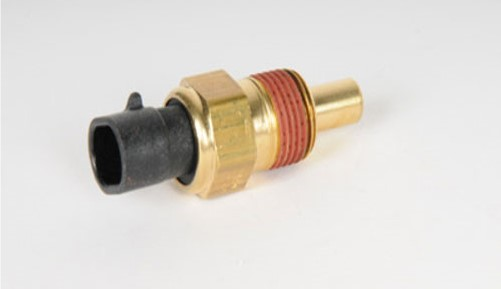
\includegraphics[]{ntc.jpg}\\
    \caption{NTC vökvahitanemi}
  \end{center}
\end{figure}
Gott er að vita hitann á kælivatni og olíu og til þess eru notuð NTC viðnám. Þau eru þeim kostum gædd að viðnám yfir þau breytast eftir því hver hitinn er. Þau eru þó ekki gallalaus þar sem viðnámsferlinum sem fall af hita er lýst eftirfarandi jöfnu, svo að 
\begin{align} 
	\begin{split}
	\frac{1}{T} = a + b \cdot ln(R) + c \cdot ln(R)^3
	\end{split}					
\end{align}
Í staðinn fyrir að eiga við hana og mæla vökvaskynjarana þá fengum við upplýsingar um þá af netinu. Fengum við viðnámið yfir viðnámin milli -30 upp í 150 í 5°C skrefum\\
Til þess að tölvan geti síðan notað þær upplýsingar þurfti að búa til uppflettitöflu. Þá lá beint við að hafa uppflettitöflu af stærðinni 256 en þá notuðum við interpolate fítus í matlab sem gerir þá línulega nálgun milli mælipunktanna, þá 256 stök milli 0 og 5v. \\
256 stök eru valin því að AD breyta stýriörgjörvans skilar 8 bita tölu á hraðri stillingu. 
\subsection{TMAP skynjari}
\begin{center}
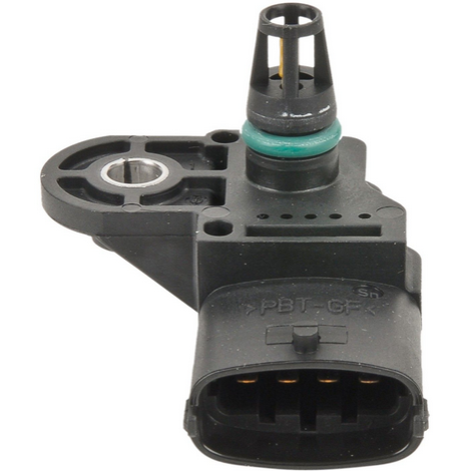
\includegraphics[scale = 0.5]{tmap.png}\\
\end{center}
TMAP skynjarinn  mælir bæði lofthita og loftþrýsting á loftinntaki. Lofthitann mælir hann með NTC viðnámi og vegna þess að það fundust engar upplýsingar um nemann þá var ákveðið að mæla viðnámið yfir hann nákvæmlega frá 120\textdegree C niður í -10\textdegree C. Til þess var arduino notaður sem spjallaði við matlab í gegnum serial samskipti, þannig var hægt að fá mjög góða upplausn á mælingum.\\
Mælingin fór þannig fram að DS18B20 I\textsuperscript{2}C hitanemi var staðsettur uppvið hitaviðnámið. Spennan yfir ntc viðnámið í raðtenginu við 1k viðnám og 5V reference spennu var mæld á sama tíma. Hitanemarnir tveir voru þá hitaðir hægt og rólega með hitabyssu og vafðir tusku. Þá var hægt að láta þá kólna hægt og rólega og tryggja þannig að þeir kólnuðu á sama hraða. Ferillinn var síðan interpolate'aður til að fá 256 stök sem pössuðu í uppflettitöflu sem stýriörgjörvinn gat notað. \\
\\
Þrýstineminn var gefinn upp 0.25V við 11kPa og 4.75V við 307kPa og línulegur þar á milli. Við prófanir voru þær tölur staðfestar og í ljós kom að um absolute þrýsting var að ræða. \\
Þá var þrýstingnum sem fall af spennu, miðað við 5V reference spennu, lýst með: 
\begin{align} 
	\begin{split}
	P=0.0438V + 0.0991 
	\end{split}					
\end{align}

\subsection{Olíuþrýstinemi}
\begin{center}
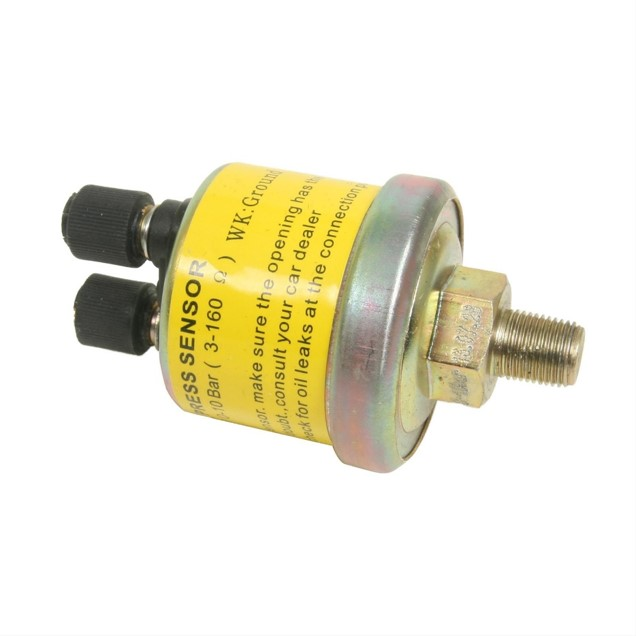
\includegraphics[scale = 0.5]{oilp.jpg} \\
\end{center}
Þá er þrýstingnum lýst með 1k$\Omega$ \space  viðnámi og 5V reference spennu:  
\begin{align} 
	\begin{split}
	P = 0.0802 V + 0.0062
	\end{split}					
\end{align}
Vegna þess hve lítið viðnámið yfir nemann er, þarf að breyta Aref spennunni í 1.1V. 
\subsection{Inngjafarstöðuskynjari}
\begin{figure}
	\begin{center}
		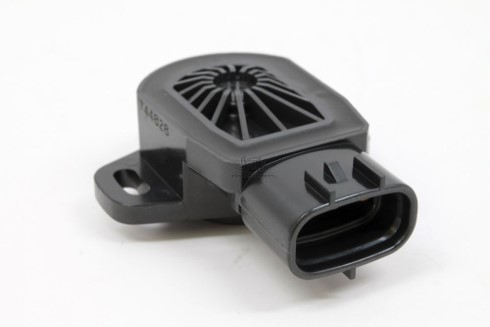
\includegraphics[]{tps.jpg}\\
        \caption{Stöðu skynjari fyrir inngjafarspjald}
	\end{center}
\end{figure}
Inngjafarstöðu skynjari eða TPS(throttle position sensor) skynjar stöðu inngjafar frá lokaðri stöðu.\\
Á Figure 3.5 má sjá mælingar sem gerðar voru á skynjararnum. Voru þá annarsvegar mældar gráðurnar á opnun frá lokaðri stöðu, þetta var gert án inngjafarspjaldsins sjálfs og mælt með gráðuboga til að áætla gráður opnunaninnar. Skynjarnann sem er í raun bara stilliviðnám í húsi, var tengdur við 5 V spennu og var spennan útaf honum mæld um leið og hann var opnaður í 10° stigum. Mælingarnar úr þessari tilraun má sjá í töflunni figure 3.5\\
Stöðuskynjari líkt og þessi er notaður í mótornum til að hjálpa til við að áætla bensín magn sem vélartölva þarf að skammta mótornum, þ.e.a.s hvort inngjöfin sé að opna eða loka og þannig hægt að áætla álag á mótorinn.
\subsection{Súrefnisskynjari}
\begin{figure}
	\begin{center}
		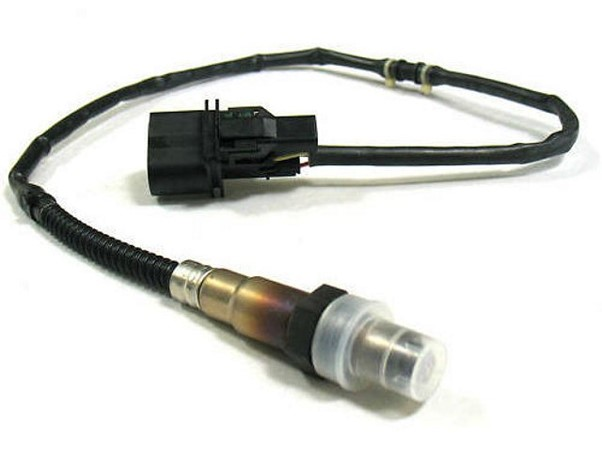
\includegraphics[]{wideband.jpg}\\
        \caption{Súrefnis skynjari}
	\end{center}
\end{figure}
Súrefnis skynjarinn er staðsettur í útblástursröri mótorsins og er notaður til að mæla hlutfall súrefnis í útblæstri mótorsins. Þannig fæst svokallað lamba-gildi sem segir til um bruna eldsneytis í brunahólfi, hvort blanda súefnis og eldsneytis sé rétt eða hvort of mikið sé af öðru hvoru. Þetta er mikilvægt að vita því vitlaus blanda getur stytt endingartíma mótorsins verulega og jafnvel skemmt hann.\\
Eftir að hafa reynt mælingar og skoðanir á netinu var ákveðið að reyna ekki að útbúa yfirfærslufall fyrir súrefnis skynjarann heldur að nota tilbúna tölvu sem sérstaklega er ætluð í að þýða merki frá súrefnis skynjaranum. Þetta var gert vegna þess hversu flókið það er að reikna þetta gildi út með mikilli nákvæmni og líka vegna þess að umrædd tölva var til staðar.

\subsection{Mælaborð}
Þegar gengið hafði verið frá skynjurum byrjaði vinna við að hanna og smíða mælaborð. Smíðinni er ekki alveg lokið en hönnunin er að mestu leiti komin. 

\section{Viðauki I - Gröf}

\begin{figure}
	\begin{center}
		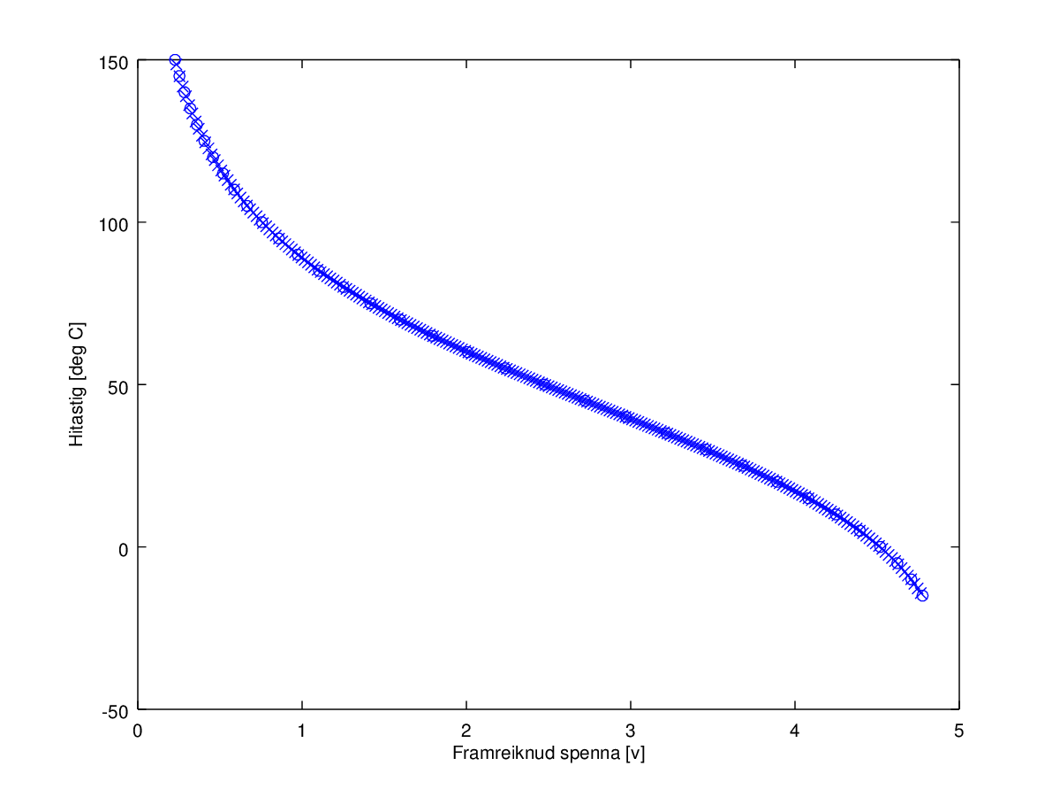
\includegraphics[scale=0.9]{NTC.png}\\
		\caption{NTC vökvahitanemi}
	\end{center}
\end{figure}
\begin{figure}
	\begin{center}
		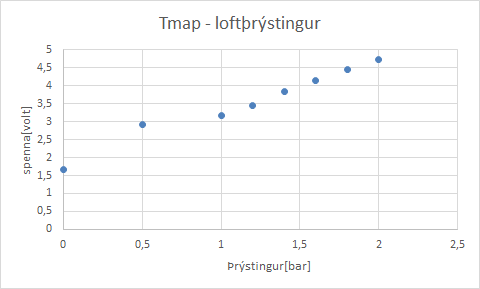
\includegraphics[]{airpress.png}\\
        \caption{Tmap loftþrýstings mæling}
	\end{center}
\end{figure}
\begin{figure}
	\begin{center}
		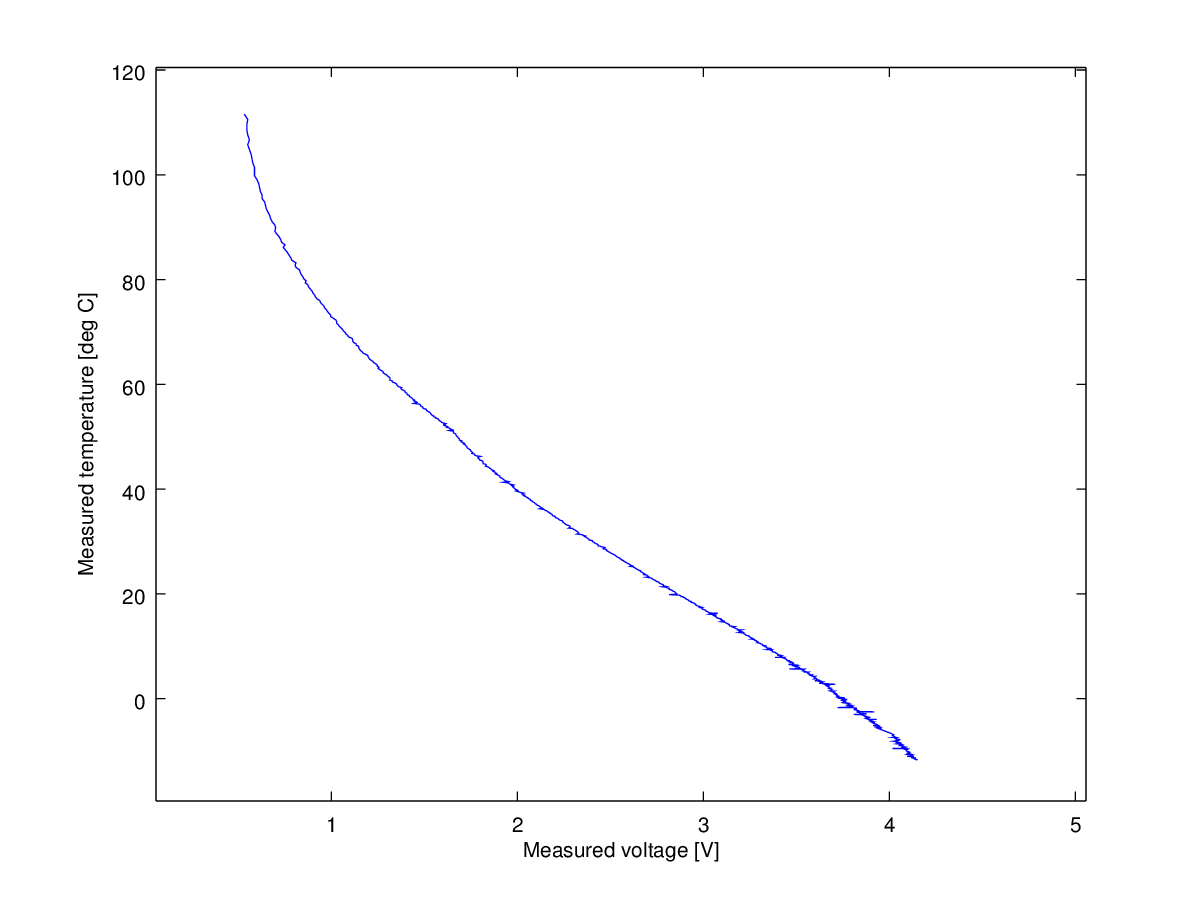
\includegraphics[scale=0.9]{tmap_temp_volts.png}\\
        \caption{Tmap hitagildis mæling}
	\end{center}
\end{figure}
\begin{figure}
	\begin{center}
		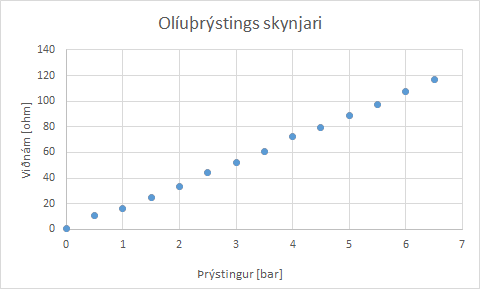
\includegraphics[]{oilpress.png}\\
        \caption{Olíuþrýstingsmælingar}
	\end{center}
\end{figure}
\begin{figure}
	\begin{center}
		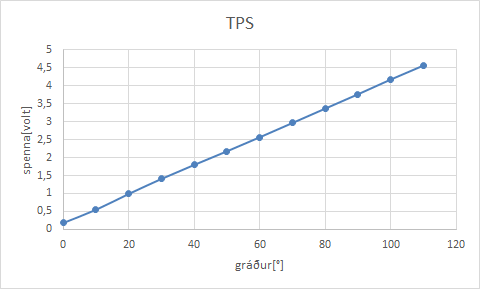
\includegraphics[]{TPS.png}\\
        \caption{Stöðuskynjara mælingar}
	\end{center}
\end{figure}
\section{Viðauki II - teikningar og layout}
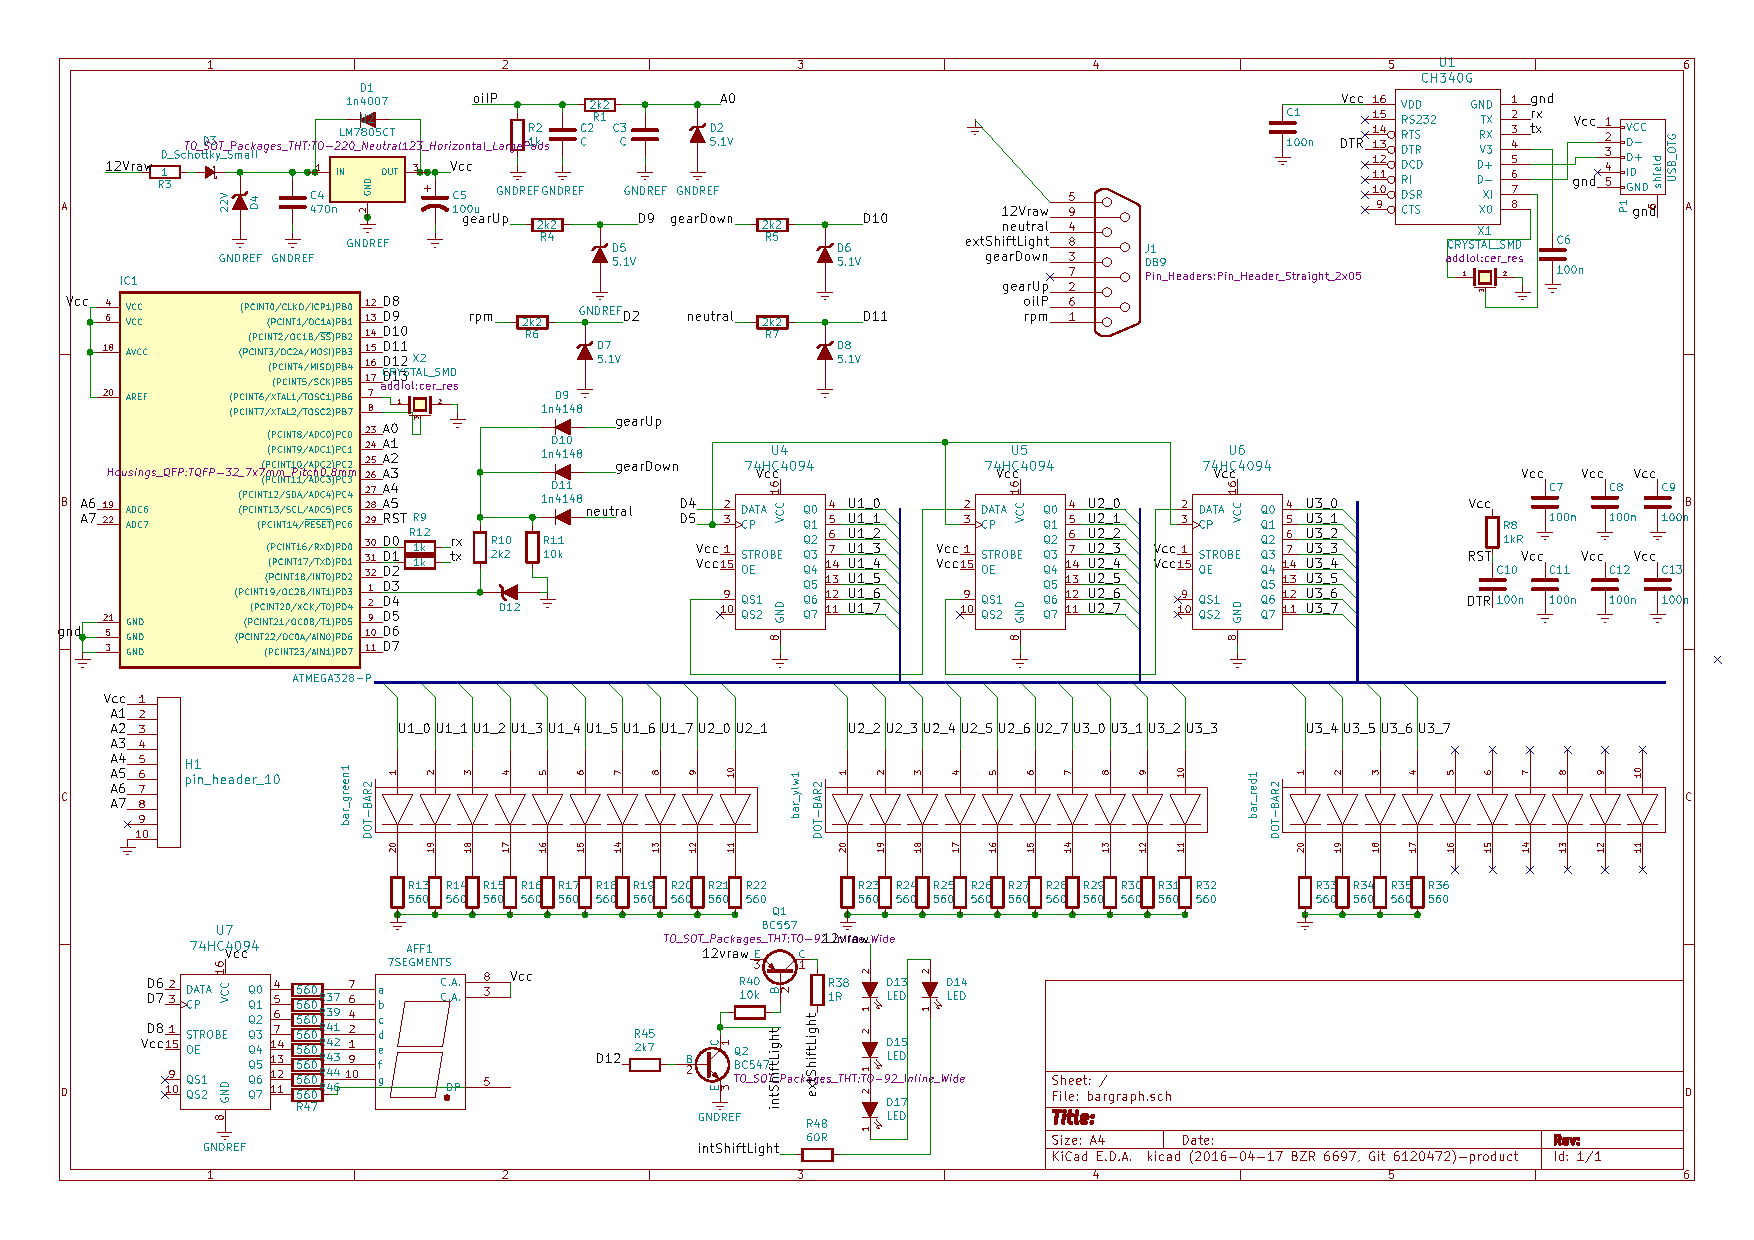
\includegraphics[angle=90, origin=c]{drawing.pdf} \\
\end{document}

